\documentclass[a4paper,12pt]{article}

\usepackage{amsmath,amsfonts,mathtools}
\usepackage{amsthm, amssymb}
\usepackage{pgfplots}
\usepackage{graphicx}
\usepackage{hyperref}
\usepackage{float}
\usepackage{subcaption}
\usepackage{enumitem}

% Personal definitions
\newcommand{\lra}{\ensuremath{\longrightarrow{}}}
\newcommand{\vect}[1]{\mathbf{#1}}
\renewcommand{\qedsymbol}{\rule{0.7em}{0.7em}}
\newcommand{\tabitem}{~~\llap{\textbullet}~~}

% Theorem commands
\newtheorem{lem}{Lemma}
\newtheorem{thm}{Theorem}
\newtheorem{defn}{Definition}

% Define a Gaussian function for plotting graphs
\pgfmathdeclarefunction{gauss}{2}{%
  \pgfmathparse{1/(#2*sqrt(2*pi))*exp(-((x-#1)^2)/(2*#2^2))}%
}

% Set version of pgfplots
\pgfplotsset{compat=1.16}

% Set spacing
\setenumerate{itemsep=1.5pt,parsep=1.5pt,topsep=0.5pt}
\setlist{itemsep=1.5pt,parsep=1.5pt,leftmargin=1pt}
\setitemize{itemsep=1.5pt,parsep=1.5pt,topsep=0.5pt}

% set 1" margins on 8.5" x 11" paper
% top left is measured from 1", 1"
\topmargin       0in
\oddsidemargin   0in
\evensidemargin  0in
\headheight      0in
\headsep         0in
\topskip         0in
\textheight      9in
\textwidth       6.5in

\begin{document}
\title{Quantum Physics I Notes}
\author{Sean Wu}
\date{\today}
\maketitle

\tableofcontents

\pagebreak

% set spacing
\setlength{\parindent}{0em}
\setlength{\parskip}{1em}

\section{Lec 1: Superposition Intuition}
\begin{itemize}
  \item Physical processes in the lab are unpredictable, nondeterminate, random
  \item Probability forced by observation

\begin{description}
  \item[Uncertainty Principle:] For incompatible properties, you cannot have an object w/ defined values for both properties at the same time
\end{description}

  \item ex. position and momentum
  \item If one property is determined, the object is in superposition of values for the other property

  \item Quantum effects negligible for large objects
  \item Quantum effects only significant for small objects w/ small energies
  \item ex. atoms, electrons, molecules
\end{itemize}

\section{Lec 2: Physical Effects explained by Quantum Mechanics but not Classical Mechanics}

\begin{enumerate}
  \item Atoms exist
  \item Randomness exists
  \item Atomic Spectra are discrete and have structure
  \item Photoelectric effect
  \item Electron Diffraction
  \item Bell's Poor Inequality
\end{enumerate}

\subsection{Atoms exist}
\begin{itemize}
  \item $e^{-}$ orbiting nucleus in Bohr atom is an accelerating charged particle and so emits light (loses energy)
  \item Thus Bohr atom doesn't work classically because it collapses as the electron spirals around nucleus while releasing energy by radiation
\end{itemize}

\subsection{Randomness exists}
\begin{itemize}
  \item Self explanatory
\end{itemize}


\subsection{Atomic Spectra}
\begin{align}
  \frac{1}{\lambda} = R \cdot \Big(\frac{1}{n_1^2} -\frac{1}{n_2^2}\Big) \text{ for } n_i \in \mathbb{Z}, n_2 > n_1
\end{align}
\begin{itemize}
  \item $R$ is the Rydberg constant which depends on the element but is independent of the emission series
  \item This eqn shows that the atomic spectra are discrete and have structure, but classical mechanics doesn't have discrete energy levels (no energy quantization)
\end{itemize}

\subsection{Photoelectric Effect}
\begin{description}
  \item[$V_0$: ] Stopping voltage req to stop $e^{-}$ from being released by photoelectric effect
  \item[$I$: ] Current generated in circuit
\end{description}

\begin{center}
  \begin{tabular}{|l|l|}
   \hline
   Prediction & Result \\
   \hline
   \tabitem More intense beam $\implies$ $e^{-}$ w/ higher KE & \tabitem  Same KE regardless of intensity\\

   \tabitem  $V_0$ $\propto$ $I$ & \tabitem $V_0$ indep of intensity\\

   \tabitem $V_0$ indep of frequnecy $\nu$ & \tabitem  $V_0$ $\propto$ $\nu$\\

   \hline
  \end{tabular}
\end{center}

\begin{itemize}
  \item Rate of $e^{-}$ release depends on intensity
  \item But for $\nu < \frac{W}{h}$ (less than critical frequency), no $e^{-}$ released regardless of intensity (not enough energy)
  \item Einstein's explanation: Light comes in chunks with defined energy $E = h\nu$
  \begin{align}
    KE = h\nu -W
  \end{align}
  where $W$ is the work required to remove the $e^{-}$
  \item Recall $E = pc$  and $c = \lambda\nu$

  \begin{align}
    \therefore{}\quad &p = \frac{h}{\lambda}
  \end{align}

  \item This implies that the discrete packets of light w/ wavelength $\lambda$ have momentum $p$ by above eqn (wave-particle duality)
\end{itemize}

\subsubsection{Waves vs Particles}
\begin{itemize}
  \item Waves can interfere with themselves (Young's Double Slit)
  \item Waves are \textbf{not localized}; particles are
  \item An interference pattern (wave) implies that \textbf{amplitudes} but intensities do not
  \item Classical particles can pass through either top or bottom slit
  \item Passing classical particles through double slit leads to 2 peaks near the 2 openings
\end{itemize}

\begin{itemize}
  \item $e^{-}$ can interfere with themselves (wave behaviour) in double slit
  \item Each $e^{-}$ takes superposition of the possible paths; We don't know if it took the top or bottom bath
  \item An $e^{-}$ is neither strictly a particle nor strictly a wave
\end{itemize}


\subsubsection{Light comes in chunks}
\begin{itemize}
  \item Light has an energy and momentum
  \begin{align}
    E &= h\nu \\
    p &= \frac{h}{\lambda}
  \end{align}
\end{itemize}

\subsection{Electron Diffraction}
\begin{itemize}
  \item Bragg's Law
  \begin{align}
    \frac{1}{\lambda} &= \frac{n}{2dsin\theta} \\
    p &= \frac{h}{\lambda}
  \end{align}
\end{itemize}

\subsection{Bell's Inequality}
\begin{itemize}
  \item For 3 binary properties A, B, C, \textbf{Bell's Inequality} states
  \begin{align}
    N(A,\overline{B}) + N(B, \overline{C}) \geq N(A, \overline{C})
  \end{align}
  where $N(X,Y)$ is the number of objects with properties X and Y
  \item $e^{-}$ have 3 binary properties (angular momentum about x-, y-, and z-axes)
  \item However, it violates Bell's Inequality
  \begin{align}
    N(\uparrow_0, \downarrow_{\theta}) + N(\uparrow_{\theta}, \downarrow_{2\theta}) \leq N(\uparrow_0, \downarrow_{2\theta})
  \end{align}
  \item Can't add probabilities classically with basic addition
\end{itemize}

\section{Lec 3: The Wave Function}

\subsection{de Broglie Relations}
\begin{equation}
  \begin{aligned}
    E &\sim \hbar & \quad\quad &E = h\nu \\
    p &= \hbar k  & \quad\quad &p = \frac{h}{\lambda}
  \end{aligned}
\end{equation}

\begin{align}
  \hbar = \frac{h}{2\pi} \quad\quad  \omega = 2\pi\nu \quad\quad k = \frac{2\pi}{\lambda}
\end{align}

\begin{description}
  \item[$\omega$ :] angular frequency [rad/s]
  \item[$k$ :] wavenumber [rad/m]
\end{description}


\subsection{Systems in Classical Mechanics vs Quantum Mechanics}
\begin{itemize}
  \item In \textbf{Classical Mechanics}, an object's state is fully defined by its position and momentum vectors $\{\vect{x}, \vect{p}\}$
  \item All other properties can be found using $\vect{x}$ and $\vect{p}$
  \item ex. energy $E(\vect{x}, \vect{p})$ and angular momentum $\vect{L}(\vect{x}, \vect{p})$
  \item But in \textbf{Quantum Mechanics} (real life), there is uncertainty (Uncertainty Principle)
  \begin{align}
    \Delta \vect{x} \Delta \vect{p} \gtrsim \hbar
  \end{align}
\end{itemize}

\subsection{Quantum Mechanics Postulates}
\begin{enumerate}
  \item The state of a quantum object is \textbf{completely} specified by a wavefunction $\Psi(x)$
  \item $\mathbb{P} = |\Psi(x)|^2$ determines the probability density that the object in state $\Psi(x)$ will be found at $x$
  \begin{itemize}
    \item i.e. probability that upon measurement, the object is found at position $x$
  \end{itemize}
  \item Given two possible wavefunctions (or states) of a quantum system corresponding to distinct wavefunctions $\Psi_1(x)$ and $\Psi_2(x)$, the system can \textbf{also} be in a \textbf{superposition} of $\Psi_1(x)$ and $\Psi_2(x)$
  \begin{align}
    \Psi(x) = \alpha\Psi_1(x) + \beta\Psi_2(x) \quad \alpha, \beta \in \mathbb{C}
  \end{align}
  such that $\Psi(x)$ is properly normalized
  \begin{itemize}
    \item Wavefunction can be expressed as a linear combination of 2 possible wavefunctions (superposition)
    \item i.e. superposition of 2 quantum states results in another valid quantum state
  \end{itemize}
\end{enumerate}

\subsection{The Wavefunction $\Psi(x)$}
\begin{itemize}
  \item Wavefunction $\Psi(x)$ is a complex function and \textbf{must} be single valued and continuous
  \item The probability $|\Psi(x)|^2$ is always real and nonnegative
  \item Probability density means

  \begin{align}
    \mathbb{P}(x, x+dx) = \mathbb{P}(x)dx = |\Psi(x)|^2dx
  \end{align}

  \item Units of wavefunction are $[\Psi(x)] = \frac{1}{\sqrt{L}}$
  \item Recall that for complex numbers,

  \begin{align}
    |\beta|^2 = \beta^* \beta \\
    |e^{i\alpha}|^2 = e^{i\alpha}e^{-i\alpha} = 1
  \end{align}

\subsection{Normalization of Wavefunctions}

  \item Probability must be \textbf{normalized} such that the sum of probabilities is 1 over an interval

  \begin{align}
    \int_{All} \mathbb{P}(x)dx = \int_{All} |\Psi(x)|^2dx = 1
  \end{align}

  \item If wave function is not normalized, then use

  \begin{align}
    \mathbb{P}(x) = \frac{|\Psi(x)|^2}{\int_{All} |\Psi(x)|^2dx}
  \end{align}

\end{itemize}

\subsection{Plane Waves}
\begin{itemize}
  \item de Broglie says a particle with energy $E \sim \hbar \omega$ and momentum $p = \hbar k$ has a plane wave wavefunction
  \item General plane wave:

  \begin{align}
    \Psi(x) = e^{i(kx-wt)}
  \end{align}
  \item Note: plane wave is a complex function (need to remember that there is an imaginary component)
  \item But not all wavefunctions are plane waves; some are well localized
\end{itemize}

\subsection{Superposition of 2 waves}
\begin{itemize}
  \item Using the rule $|\beta|^2 = \beta^* \beta$, the probability with superposition is:
  \begin{align}
    \mathbb{P} &= |\alpha\Psi_1 + \beta\Psi_2|^2 = (\alpha^*\Psi_1^* + \beta^*\Psi_2^*)(\alpha\Psi_1 + \beta\Psi_2) \\ &=|\alpha|^2|\Psi_1|^2 + |\beta|^2|\Psi_2|^2 + \alpha^*\Psi_1^* \beta\Psi_2 + \alpha\Psi_1 \beta^*\Psi_2^* \\
    &= \mathbb{P}_1 + \mathbb{P}_2 + \alpha^*\Psi_1^* \beta\Psi_2 + \alpha\Psi_1 \beta^*\Psi_2^*
  \end{align}
  where $\alpha^*\Psi_1^* \beta\Psi_2 + \alpha\Psi_1 \beta^*\Psi_2^*$ are the \textbf{interference terms}

  \item The first term in the interference terms is the conjugate of the 2\textsuperscript{nd} term
  \item Therefore the interference term is real but not necessarily nonnegative, so the overall probability will still be real
  \item Note: Superposition principle and interpretation of probability as $|\Psi(x)|^2$ gives correction to classical probability (the interference terms)
  \item Shows that probabilities don't add as they do classically in Bell's Inequality (i.e. probability of both is \textbf{not} the sum of the individual probabilities)
\end{itemize}

\textbf{Wavefunctions add; probabilities do not}

\subsection{Superposition of many waves}
\begin{itemize}
  \item As you add more plane waves to a superposition, the wavefunction and probability distribution become more localized (i.e. $\Delta x$ decreases)
  \item For lots of plane waves, get a very narrow probability distribution and wavefunction
  \item There will be very few peaks, so particle is very likely to be found at those positions: $\Delta x \sim \text{small}$
  \item But that requires a superposition of many momenta (each plane wave has a different $\lambda$ and $p = \frac{h}{\lambda}$) so $\Delta p \sim \text{large}$ as required by the Uncertainty Principle

\end{itemize}

\subsubsection{Fourier Transforms for wave functions}
\begin{thm}
  Any well behaved $f(x)$ can be built by superimposing enough plane waves $e^{ikx}$

  \begin{align}
    f(x) = \frac{1}{\sqrt{2\pi}} \int^{\infty}_{-\infty}\widetilde{f}(k) e^{ikx} dk
  \end{align}
\end{thm}
where $\widetilde{f}(x)$ gives the amplitude of the plane wave with wavelength $\lambda = \frac{2\pi}{k}$

\begin{itemize}
  \item Every mode has a definite wavelength $\lambda = \frac{2\pi}{k}$
  \item Note: Fourier Transform coefficients of $x$ are all equivalent
  \item Can use Inverse Fourier Transform to get $\widetilde{f}(k)$ from $f(x)$
  \begin{align}
    \widetilde{f}(k) = \frac{1}{\sqrt{2\pi}} \int^{\infty}_{-\infty}f(x) e^{-ikx} dx
  \end{align}
\end{itemize}

\begin{itemize}
  \item Physics Version: any $\Psi(x)$ can be expressed as the superposition of states with definite momentum $p = \hbar k$
  \begin{align}
    \Psi(x) = \frac{1}{\sqrt{2\pi}} \int^{\infty}_{-\infty}\widetilde{\Psi}(x) e^{ikx} dk
  \end{align}
  \item The Fourier Transform associates a magnitude and phase for each possible wave vector
  \item Note: if the wavefunction is well localized to a position, the Fourier Transform is not well localized ($\therefore$ not having definite momentum)
  \item Similarly, if there is definite momentum, position is not well defined, but the Fourier Transform will have a single peak (position very localized)

\end{itemize}

\subsection{Probability density for Wavenumber/Momentum}

\begin{itemize}
  \item Similar to probability density for position $x$, the probability density for momentum $p$/wavenumber $k$ is given by the norm squared of the wavefunction in the k-space
  \begin{align}
    \mathbb{P}(k) = |\Psi(k)|^2
  \end{align}
\end{itemize}



\subsection{Wavefunction Examples}

\subsubsection{Gaussian Wavefunctions}

\begin{center}

\begin{minipage}{.47\textwidth}
  \begin{align}
    \Psi(x) = \frac{1}{0.5 \sqrt{2\pi}}exp\Big(-\frac{(x+3)^2}{2\cdot 0.5}\Big)
  \end{align}
  \begin{tikzpicture}
  \begin{axis}[
    every axis plot post/.append style={mark=none,domain=-5:5,samples=50,smooth}, % All plots: from -10:10, 50 samples, smooth, no marks
    axis lines=middle,
    ylabel = $\mathbb{R}\text{e}(\Psi)$,
    xlabel = $x$,
    x label style={at=(current axis.right of origin), anchor=west},
    y label style={at=(current axis.above origin), anchor=south},
    xtick={-3},
    xticklabels={$x_1$},
    ytick=\empty]
    \addplot[color=blue]{gauss(-3,0.5)};
  \end{axis}
\end{tikzpicture}
\captionof{figure}{Ex. Gaussian Wavefunction}
%
\begin{align}
  x &\sim x_1  \\
  \Delta x &\sim \text{small}
\end{align}
%
\end{minipage}
%
\begin{minipage}{.47\textwidth}
  \begin{align}
    \Psi(x) = \frac{1}{0.5 \sqrt{2\pi}}exp\Big(-\frac{(x-2.5)^2}{2\cdot 0.5}\Big)
  \end{align}
  \begin{tikzpicture}
  \begin{axis}[
    every axis plot post/.append style={mark=none,domain=-5:5,samples=50,smooth}, % All plots: from -10:10, 50 samples, smooth, no marks
    axis lines=middle,
    ylabel = $\mathbb{R}\text{e}(\Psi)$,
    xlabel = $x$,
    x label style={at=(current axis.right of origin), anchor=west},
    y label style={at=(current axis.above origin), anchor=south},
    xtick={2.5},
    xticklabels={$x_2$},
    ytick=\empty]
    \addplot[color=red]{gauss(2.5,0.5)};
  \end{axis}
\end{tikzpicture}
\captionof{figure}{Ex. Gaussian Wavefunction }
%
\begin{align}
  x &\sim x_2  \\
  \Delta x &\sim \text{small}
\end{align}
%
\end{minipage}
\end{center}

\begin{itemize}
  \item For both Gaussian wavefunctions above, there is no definite wavelength, so $\Delta p \sim {large}$
\end{itemize}

\begin{center}

\begin{minipage}{.47\textwidth}
  \begin{tikzpicture}
  \begin{axis}[
    every axis plot post/.append style={mark=none,domain=-5:5,samples=50,smooth}, % All plots: from -10:10, 50 samples, smooth, no marks
    axis lines=middle,
    ylabel = $\mathbb{P}(x)$,
    xlabel = $x$,
    x label style={at=(current axis.right of origin), anchor=west},
    y label style={at=(current axis.above origin), anchor=south},
    xtick={-3},
    xticklabels={$x_1$},
    ytick=\empty]
    \addplot[color=blue]{gauss(-3,0.5)^2};
  \end{axis}
\end{tikzpicture}
\captionof{figure}{Probability density}
\end{minipage}
%
\begin{minipage}{.47\textwidth}
  \begin{tikzpicture}
  \begin{axis}[
    every axis plot post/.append style={mark=none,domain=-5:5,samples=50,smooth}, % All plots: from -10:10, 50 samples, smooth, no marks
    axis lines=middle,
    ylabel = $\mathbb{P}(x)$,
    xlabel = $x$,
    x label style={at=(current axis.right of origin), anchor=west},
    y label style={at=(current axis.above origin), anchor=south},
    xtick={2.5},
    xticklabels={$x_2$},
    ytick=\empty]
    \addplot[color=red]{gauss(2.5,0.5)^2};
  \end{axis}
\end{tikzpicture}
\captionof{figure}{Probability density}
\end{minipage}
\end{center}

\begin{center}

\begin{minipage}{.47\textwidth}
  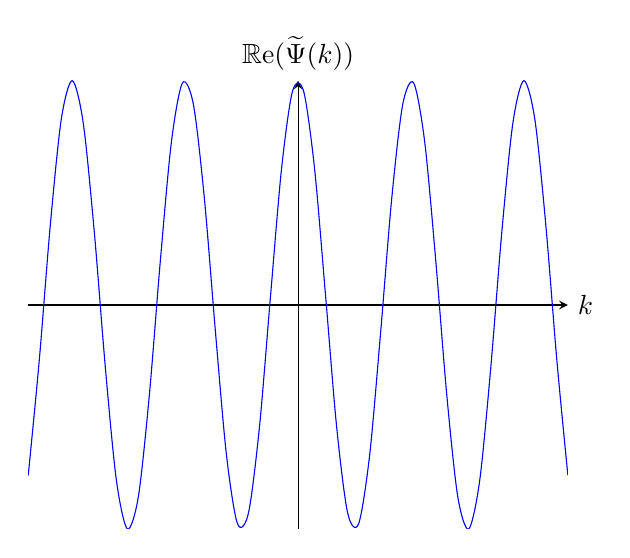
\begin{tikzpicture}
  \begin{axis}[
    every axis plot post/.append style={mark=none,domain=-5:5,samples=50,smooth}, % All plots: from -10:10, 50 samples, smooth, no marks
    axis lines=middle,
    ylabel = $\mathbb{R}\text{e}(\widetilde{\Psi}(k))$,
    xlabel = $k$,
    x label style={at=(current axis.right of origin), anchor=west},
    y label style={at=(current axis.above origin), anchor=south},
    xtick=\empty,
    ytick=\empty]
    \addplot[color=blue]{cos(deg(3*x))};
  \end{axis}
\end{tikzpicture}
\captionof{figure}{Wavefunction in k-space}
%
\begin{align}
  p &\sim \text{???} \\
  \Delta p &\sim {large}
\end{align}
%
\end{minipage}
%
\begin{minipage}{.47\textwidth}
  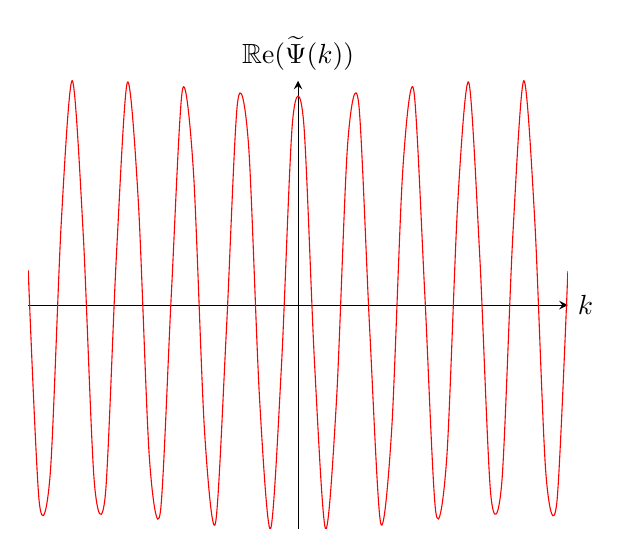
\begin{tikzpicture}
  \begin{axis}[
    every axis plot post/.append style={mark=none,domain=-5:5,samples=50,smooth}, % All plots: from -10:10, 50 samples, smooth, no marks
    axis lines=middle,
    ylabel = $\mathbb{R}\text{e}(\widetilde{\Psi}(k))$,
    xlabel = $k$,
    x label style={at=(current axis.right of origin), anchor=west},
    y label style={at=(current axis.above origin), anchor=south},
    xtick=\empty,
    ytick=\empty]
    \addplot[color=red]{cos(deg(6*x))};
  \end{axis}
\end{tikzpicture}
\captionof{figure}{Wavefunction in k-space}
%
\begin{align}
  p &\sim \text{???} \\
  \Delta p &\sim {large}
\end{align}
%
\end{minipage}
\end{center}

\begin{center}

\begin{minipage}{.47\textwidth}
  \begin{tikzpicture}
  \begin{axis}[
    every axis plot post/.append style={mark=none,domain=-5:5,samples=50,smooth}, % All plots: from -10:10, 50 samples, smooth, no marks
    axis lines=middle,
    ylabel = $\mathbb{P}(k)$,
    xlabel = $k$,
    x label style={at=(current axis.right of origin), anchor=west},
    y label style={at=(current axis.above origin), anchor=south},
    xtick=\empty,
    ytick={1},
    yticklabels={1}]
    \addplot[color=blue]{1};
  \end{axis}
\end{tikzpicture}
\captionof{figure}{Probability density of wavefunction having specific wavenumbers $k$}
\end{minipage}
%
\begin{minipage}{.47\textwidth}
  \begin{tikzpicture}
  \begin{axis}[
    every axis plot post/.append style={mark=none,domain=-5:5,samples=50,smooth}, % All plots: from -10:10, 50 samples, smooth, no marks
    axis lines=middle,
    ylabel = $\mathbb{P}(k)$,
    xlabel = $k$,
    x label style={at=(current axis.right of origin), anchor=west},
    y label style={at=(current axis.above origin), anchor=south},
    xtick=\empty,
    ytick={1},
    yticklabels={1}]
    \addplot[color=red]{1};
  \end{axis}
\end{tikzpicture}
\captionof{figure}{Probability density of wavefunction having specific wavenumbers $k$}
\end{minipage}
\end{center}

\subsubsection{Plane Waves (Complex Exponential Form)}


\begin{center}

\begin{minipage}{.47\textwidth}
  \begin{align}
    \Psi(x) = -e^{i k_1 x}
  \end{align}
  \begin{tikzpicture}
  \begin{axis}[
    every axis plot post/.append style={mark=none,domain=-5:5,samples=50,smooth}, % All plots: from -10:10, 50 samples, smooth, no marks
    axis lines=middle,
    ylabel = $\mathbb{R}\text{e}(\Psi)$,
    xlabel = $x$,
    x label style={at=(current axis.right of origin), anchor=west},
    y label style={at=(current axis.above origin), anchor=south},
    xtick=\empty,
    ytick=\empty]
    \addplot[color=blue]{-cos(deg(x))};
  \end{axis}
\end{tikzpicture}
\captionof{figure}{Ex. Plane Wavefunction}
%
\begin{align}
  x &\sim \text{???} \\
  \Delta x &\sim \text{large} \\
\end{align}
%
\end{minipage}
%
\begin{minipage}{.47\textwidth}
  \begin{align}
    \Psi(x) = e^{i k_2 x}
  \end{align}
  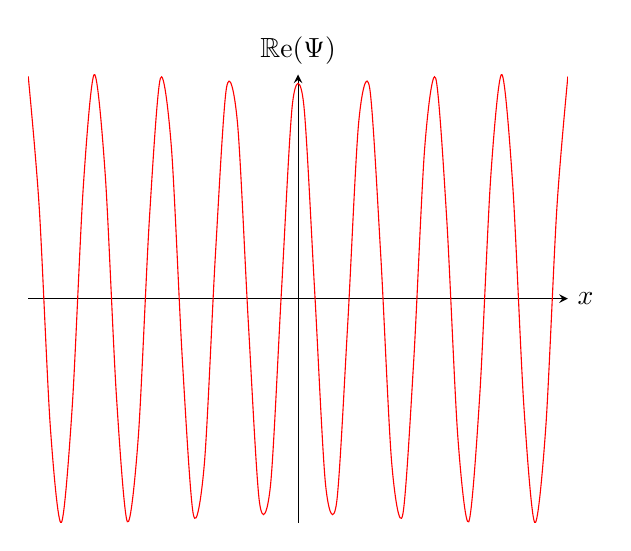
\begin{tikzpicture}
  \begin{axis}[
    every axis plot post/.append style={mark=none,domain=-5:5,samples=50,smooth}, % All plots: from -10:10, 50 samples, smooth, no marks
    axis lines=middle,
    ylabel = $\mathbb{R}\text{e}(\Psi)$,
    xlabel = $x$,
    x label style={at=(current axis.right of origin), anchor=west},
    y label style={at=(current axis.above origin), anchor=south},
    xtick=\empty,
    ytick=\empty]
    \addplot[color=red]{cos(deg(5*x))};
  \end{axis}
\end{tikzpicture}
\captionof{figure}{Ex. Plane Wavefunction }
%
\begin{align}
  x &\sim \text{???}  \\
  \Delta x &\sim \text{large}
\end{align}
%
\end{minipage}
\end{center}

\begin{center}

\begin{minipage}{.47\textwidth}
  \begin{tikzpicture}
  \begin{axis}[
    every axis plot post/.append style={mark=none,domain=-5:5,samples=50,smooth}, % All plots: from -10:10, 50 samples, smooth, no marks
    axis lines=middle,
    ylabel = $\mathbb{P}(x)$,
    xlabel = $x$,
    x label style={at=(current axis.right of origin), anchor=west},
    y label style={at=(current axis.above origin), anchor=south},
    xtick=\empty,
    ytick={1},
    yticklabels={1}]
    \addplot[color=blue]{1};
  \end{axis}
\end{tikzpicture}
\captionof{figure}{Probability density}
\end{minipage}
%
\begin{minipage}{.47\textwidth}
  \begin{tikzpicture}
  \begin{axis}[
    every axis plot post/.append style={mark=none,domain=-5:5,samples=50,smooth}, % All plots: from -10:10, 50 samples, smooth, no marks
    axis lines=middle,
    ylabel = $\mathbb{P}(x)$,
    xlabel = $x$,
    x label style={at=(current axis.right of origin), anchor=west},
    y label style={at=(current axis.above origin), anchor=south},
    xtick=\empty,
    ytick={1},
    yticklabels={1}]
    \addplot[color=red]{1};
  \end{axis}
\end{tikzpicture}
\captionof{figure}{Probability density}
\end{minipage}
\end{center}

\begin{itemize}
  \item Note: wavefunction is not properly normalized
  \item Particle can be anywhere ($\Delta x \sim \text{large}$)
  \item But $\Psi(x)$ has a very defined wavelength and wavenumber, so the particle has a defined momentum $p = \hbar k$
\end{itemize}


\begin{center}

\begin{minipage}{.47\textwidth}
  \begin{tikzpicture}
  \begin{axis}[
    every axis plot post/.append style={mark=none,domain=-5:5,samples=50,smooth}, % All plots: from -10:10, 50 samples, smooth, no marks
    axis lines=middle,
    ylabel = $\mathbb{R}\text{e}(\widetilde{\Psi}(k))$,
    xlabel = $k$,
    x label style={at=(current axis.right of origin), anchor=west},
    y label style={at=(current axis.above origin), anchor=south},
    xtick={-1},
    xticklabels={$k_1$},
    ytick=\empty]
    \addplot[color=blue]{gauss(-1,0.5)};
  \end{axis}
\end{tikzpicture}
\captionof{figure}{Wavefunction in k-space}
\end{minipage}
%
\begin{minipage}{.47\textwidth}
  \begin{tikzpicture}
  \begin{axis}[
    every axis plot post/.append style={mark=none,domain=-5:5,samples=50,smooth}, % All plots: from -10:10, 50 samples, smooth, no marks
    axis lines=middle,
    ylabel = $\mathbb{R}\text{e}(\widetilde{\Psi}(k))$,
    xlabel = $k$,
    x label style={at=(current axis.right of origin), anchor=west},
    y label style={at=(current axis.above origin), anchor=south},
    xtick={3},
    xticklabels={$k_2$},
    ytick=\empty]
    \addplot[color=red]{gauss(3,0.5)};
  \end{axis}
\end{tikzpicture}
\captionof{figure}{Wavefunction in k-space}
\end{minipage}
\end{center}

\begin{center}

\begin{minipage}{.47\textwidth}
  \begin{tikzpicture}
  \begin{axis}[
    every axis plot post/.append style={mark=none,domain=-5:5,samples=50,smooth}, % All plots: from -10:10, 50 samples, smooth, no marks
    axis lines=middle,
    ylabel = $\mathbb{P}(k)$,
    xlabel = $k$,
    x label style={at=(current axis.right of origin), anchor=west},
    y label style={at=(current axis.above origin), anchor=south},
    xtick={-1},
    xticklabels={$k_1$},
    ytick=\empty]
    \addplot[color=blue]{gauss(-1,0.5)^2};
  \end{axis}
\end{tikzpicture}
\captionof{figure}{Probability density of wavefunction having specific wavenumbers $k$}
%
\begin{align}
  p &\sim \hbar k_1 \\
  \Delta p &\sim {small}
\end{align}
%
\end{minipage}
%
\begin{minipage}{.47\textwidth}
  \begin{tikzpicture}
  \begin{axis}[
    every axis plot post/.append style={mark=none,domain=-5:5,samples=50,smooth}, % All plots: from -10:10, 50 samples, smooth, no marks
    axis lines=middle,
    ylabel = $\mathbb{P}(k)$,
    xlabel = $k$,
    x label style={at=(current axis.right of origin), anchor=west},
    y label style={at=(current axis.above origin), anchor=south},
    xtick={3},
    xticklabels={$k_2$},
    ytick=\empty]
    \addplot[color=red]{gauss(3,0.5)^2};
  \end{axis}
\end{tikzpicture}
\captionof{figure}{Probability density of wavefunction having specific wavenumbers $k$}
%
\begin{align}
  p &\sim \hbar k_2 \\
  \Delta p &\sim {small}
\end{align}
%
\end{minipage}
\end{center}


\subsubsection{Superposition of 2 Wavefunctions}

\begin{center}

  \begin{minipage}{.47\textwidth}
    \begin{align}
      \Psi(x) = \frac{1}{4}\frac{1}{0.5 \sqrt{2\pi}}exp\Big(-\frac{(x+3)^2}{2\cdot 0.5}\Big) \\
       + \frac{3}{4}\frac{1}{0.5 \sqrt{2\pi}}exp\Big(-\frac{(x-2.5)^2}{2\cdot 0.5}\Big)
    \end{align}
    \begin{tikzpicture}
    \begin{axis}[
      every axis plot post/.append style={mark=none,domain=-5:5,samples=50,smooth}, % All plots: from -10:10, 50 samples, smooth, no marks
      axis lines=middle,
      ylabel = $\mathbb{R}\text{e}(\Psi)$,
      xlabel = $x$,
      x label style={at=(current axis.right of origin), anchor=west},
      y label style={at=(current axis.above origin), anchor=south},
      xtick={-3,1,2.5},
      xticklabels={$x_1$,$x_{avg}$,$x_2$},
      ytick=\empty]
      \addplot[color=blue]{0.25*gauss(-3,0.5)+ gauss(2.5,0.5)};
    \end{axis}
  \end{tikzpicture}
  \captionof{figure}{Ex. Superposition of 2 Gaussian Wavefunctions}
  %
  \begin{align}
    x &\sim \text{in betw } x_1 \text{ and } x_2 \text{ on avg}  \\
    \Delta x &\sim (x_1 - x_2)
  \end{align}
  %
  \end{minipage}
  %
  \begin{minipage}{.47\textwidth}
    \begin{align}
      \Psi(x) &= e^{i k_1 x} + e^{i k_2 x} \\ &= -e^{ix} + 0.25e^{5ix}
    \end{align}
    \begin{tikzpicture}
    \begin{axis}[
      every axis plot post/.append style={mark=none,domain=-5:5,samples=50,smooth}, % All plots: from -10:10, 50 samples, smooth, no marks
      axis lines=middle,
      ylabel = $\mathbb{R}\text{e}(\Psi)$,
      xlabel = $x$,
      x label style={at=(current axis.right of origin), anchor=west},
      y label style={at=(current axis.above origin), anchor=south},
      xtick=\empty,
      ytick=\empty]
      \addplot[color=red]{-cos(deg(x))+0.25*cos(deg(5*x))};
    \end{axis}
  \end{tikzpicture}
  \captionof{figure}{Ex. Superpositions of 2 Plane Wavefunctions}
  %
  \begin{align}
    x &\sim \text{some info}  \\
    \Delta x &\sim \text{huge}
  \end{align}
  %
  \end{minipage}
  \end{center}

\begin{center}
  \begin{minipage}{.47\textwidth}
    \begin{tikzpicture}
    \begin{axis}[
      every axis plot post/.append style={mark=none,domain=-5:5,samples=50,smooth}, % All plots: from -10:10, 50 samples, smooth, no marks
      axis lines=middle,
      ylabel = $\mathbb{P}(x)$,
      xlabel = $x$,
      x label style={at=(current axis.right of origin), anchor=west},
      y label style={at=(current axis.above origin), anchor=south},
      xtick={-3,1,2.5},
      xticklabels={$x_1$,$x_{avg}$,$x_2$},
      ytick=\empty]
      \addplot[color=blue]{(0.25*gauss(-3,0.5)+gauss(2.5,0.5))^2};
    \end{axis}
  \end{tikzpicture}
  \captionof{figure}{Probability density}
  \end{minipage}
  %
  \begin{minipage}{.47\textwidth}
    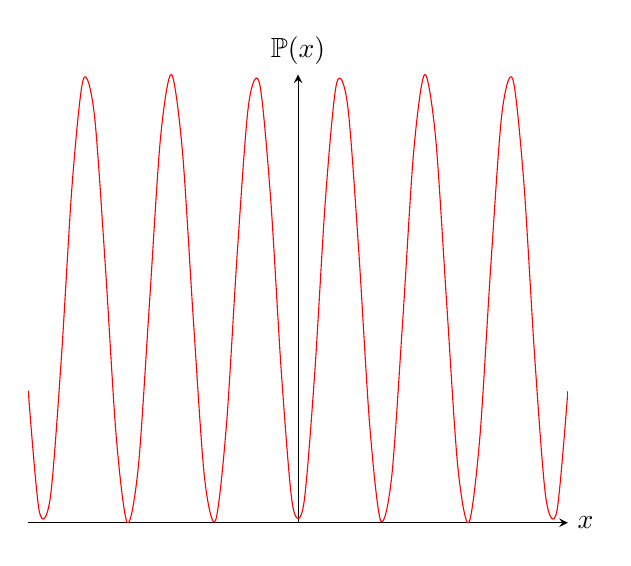
\begin{tikzpicture}
    \begin{axis}[
      every axis plot post/.append style={mark=none,domain=-5:5,samples=50,smooth}, % All plots: from -10:10, 50 samples, smooth, no marks
      axis lines=middle,
      ylabel = $\mathbb{P}(x)$,
      xlabel = $x$,
      x label style={at=(current axis.right of origin), anchor=west},
      y label style={at=(current axis.above origin), anchor=south},
      xtick=\empty,
      ytick=\empty]
      \addplot[color=red]{17/16 -0.5*cos(deg(4*x))};
    \end{axis}
  \end{tikzpicture}
  \captionof{figure}{Probability density}
  \end{minipage}
  \end{center}

  \begin{center}

  \begin{minipage}{.47\textwidth}
    \begin{align}
      \Psi(x) &= e^{i k x_1} + e^{i k x_2} \\ &= e^{ix} + 0.3e^{5ix}
    \end{align}
    \begin{tikzpicture}
    \begin{axis}[
      every axis plot post/.append style={mark=none,domain=-5:5,samples=50,smooth}, % All plots: from -10:10, 50 samples, smooth, no marks
      axis lines=middle,
      ylabel = $\mathbb{R}\text{e}(\widetilde{\Psi}(k))$,
      xlabel = $k$,
      x label style={at=(current axis.right of origin), anchor=west},
      y label style={at=(current axis.above origin), anchor=south},
      xtick=\empty,
      ytick=\empty]
      \addplot[color=blue]{cos(deg(x)) + 0.3*cos(deg(5*x))};
    \end{axis}
  \end{tikzpicture}
  \captionof{figure}{Wavefunction in k-space}
  \end{minipage}
  %
  \begin{minipage}{.47\textwidth}
    \begin{align}
      \Psi(x) = \frac{1}{4}\frac{1}{0.5 \sqrt{2\pi}}exp\Big(-\frac{(x+3)^2}{2\cdot 0.5}\Big) \\
       + \frac{1}{0.5 \sqrt{2\pi}}exp\Big(-\frac{(x-2.5)^2}{2\cdot 0.5}\Big)
    \end{align}
    \begin{tikzpicture}
    \begin{axis}[
      every axis plot post/.append style={mark=none,domain=-5:5,samples=50,smooth}, % All plots: from -10:10, 50 samples, smooth, no marks
      axis lines=middle,
      ylabel = $\mathbb{R}\text{e}(\widetilde{\Psi}(k))$,
      xlabel = $k$,
      x label style={at=(current axis.right of origin), anchor=west},
      y label style={at=(current axis.above origin), anchor=south},
      xtick={-3, 2.5},
      xticklabels={$k_1$,$k_2$},
      ytick=\empty]
      \addplot[color=red]{0.25*gauss(-3,0.5)+gauss(2.5,0.5};
    \end{axis}
  \end{tikzpicture}
  \captionof{figure}{Wavefunction in k-space}
  \end{minipage}
\end{center}


\section{Aside: More about Fourier Transforms}

\subsection{Fourier Series}
\begin{itemize}
  \item Can represent any periodic function $f(x)$ with a Fourier series

  \begin{align}
    f(x) = \frac{1}{2}a_0 + \sum^{\infty}_{n=1} a_n cos(nx) + \sum^{\infty}_{n=1} b_n sin(nx)
  \end{align}


  \begin{figure}[H]
    \centering
    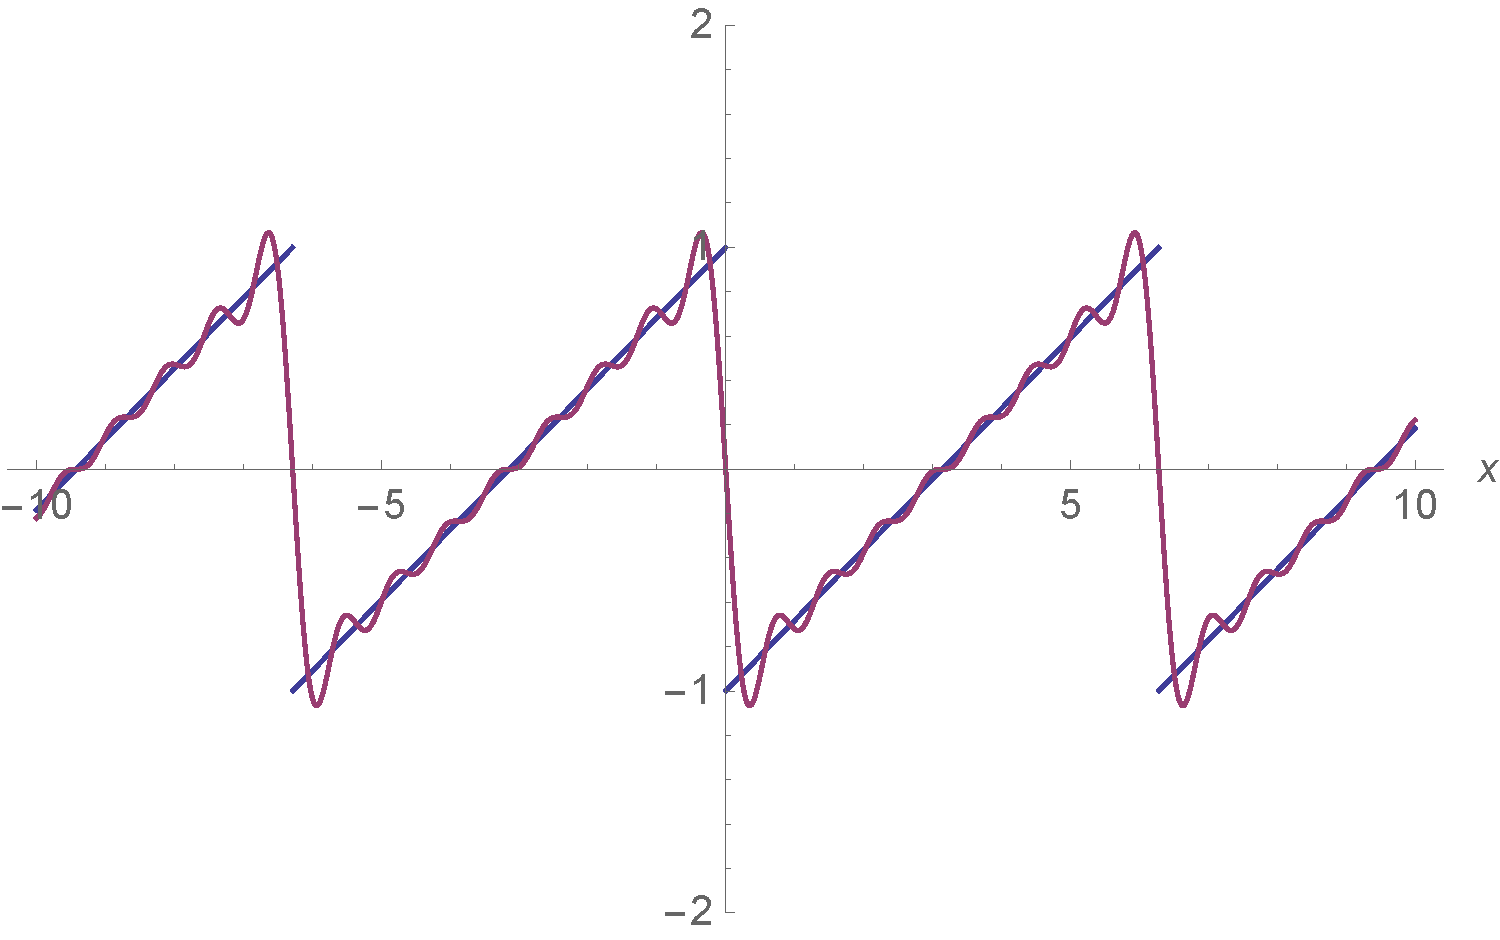
\includegraphics[width=140mm, scale=0.5]{images/sawtooth.pdf}
    \caption{Graph of a periodic sawtooth function in the real x-space}
    \label{Basic-Sawtooth}
  \end{figure}


\subsection{Fourier k-space (Frequency domain)}

  \item Can also describe the Fourier representation by plotting the strength of each sine/cosine term as a function of frequency/wavenumber (k), $\widetilde{f}(k)$
  \item Frequency representation is obtained by applying the Fourier Transform to the original function in the time domain

  \begin{itemize}
    \item Wavenumber used as dependent variable on x-axis
    \item Fourier coefficients $a_n$ or $b_n$ are then used as the amplitude of each wavenumber
  \end{itemize}
\end{itemize}

\begin{figure}[H]
  \centering
  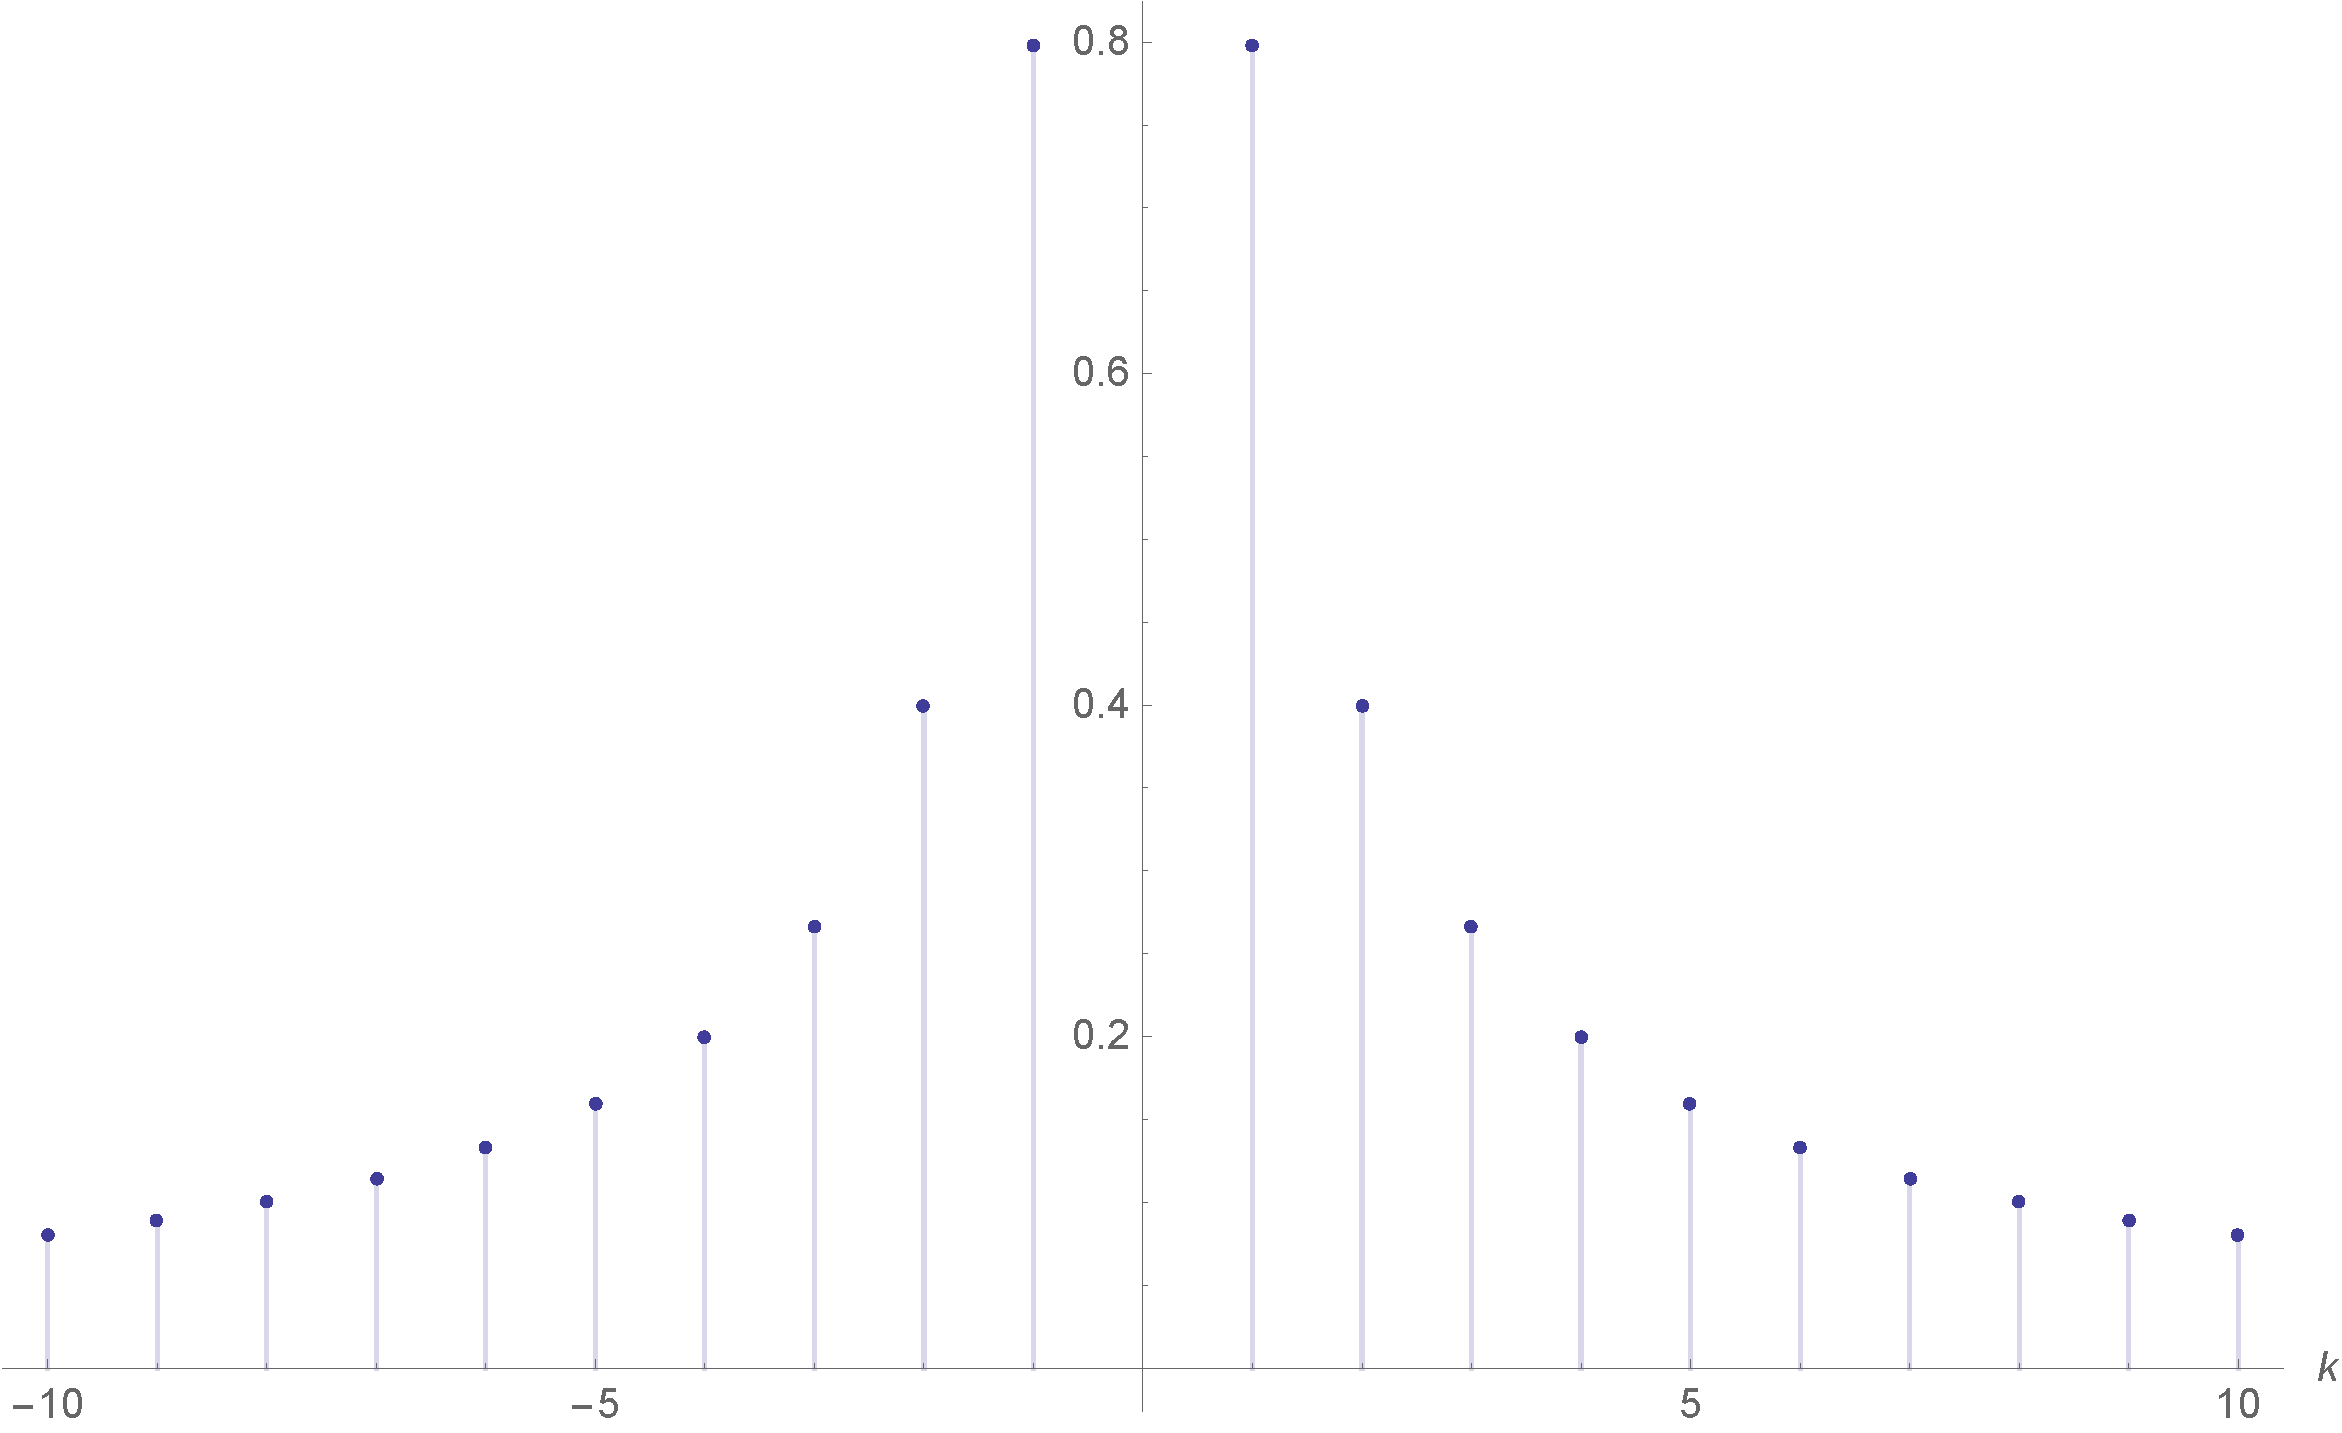
\includegraphics[width=140mm, scale=0.5]{images/sawtooth-k-space.pdf}
  \caption{Graph of a periodic sawtooth function in Fourier k-space}
  \label{Sawtooth-k-space}
\end{figure}

\begin{itemize}
  \item For the Fourier Transform of the sawtooth function, the k-space graph has discrete nonzero values for only specific wavenumbers, which means that "in-between" frequencies/wavenumbers are not needed
  \item Note: amplitude of the function is large for small wavenumbers $k$ and decreases for larger $k$
  \item Therefore, high frequency terms can be considered negligible (can approximate Fourier series with the first few terms)
\end{itemize}

\subsection{How Period Length affects the Fourier Transform}

\begin{itemize}
  \item Can represent any function in the "real x-space" (wiggly function) or in the "Fourier k-space" (spiky function)
  \item The shorter the period of the original function, the sparser the Fourier representation; i.e. less wavenumbers required (Red sawtooth function)
  \item The longer the period, the denser the Fourier representation (Blue sawtooth function)
  \begin{itemize}
    \item The main contributing wavenumbers are condensed centrally closer to the small k-values
    \item Since $k = \frac{2\pi}{\lambda} = \frac{2\pi}{c T}$, $k \sim \frac{1}{T}$
    \item So if the original function has a longer period $T$, its Fourier series needs sinusoids with longer periods (smaller $k$)
    \item i.e. the more "stretched out" a function is in the real space (longer period), the more centralized/"squished" it is in the Fourier space
  \end{itemize}
  \item Note: "periodic" functions with infinite period are aperiodic functions (never repeats itself)
  \item As the period approaches infinity, spikes in the k-space get infinitely squished together and form a continuous function
  \item Therefore, while a periodic function can be represented by a discrete set of sines and cosines (only some wavenumbers), an aperiodic function (most functions) can only be formed from a \textbf{continuous} sum of sines and cosines (include all intermediate wavenumbers)
\end{itemize}

\begin{figure}[H]
  \centering
  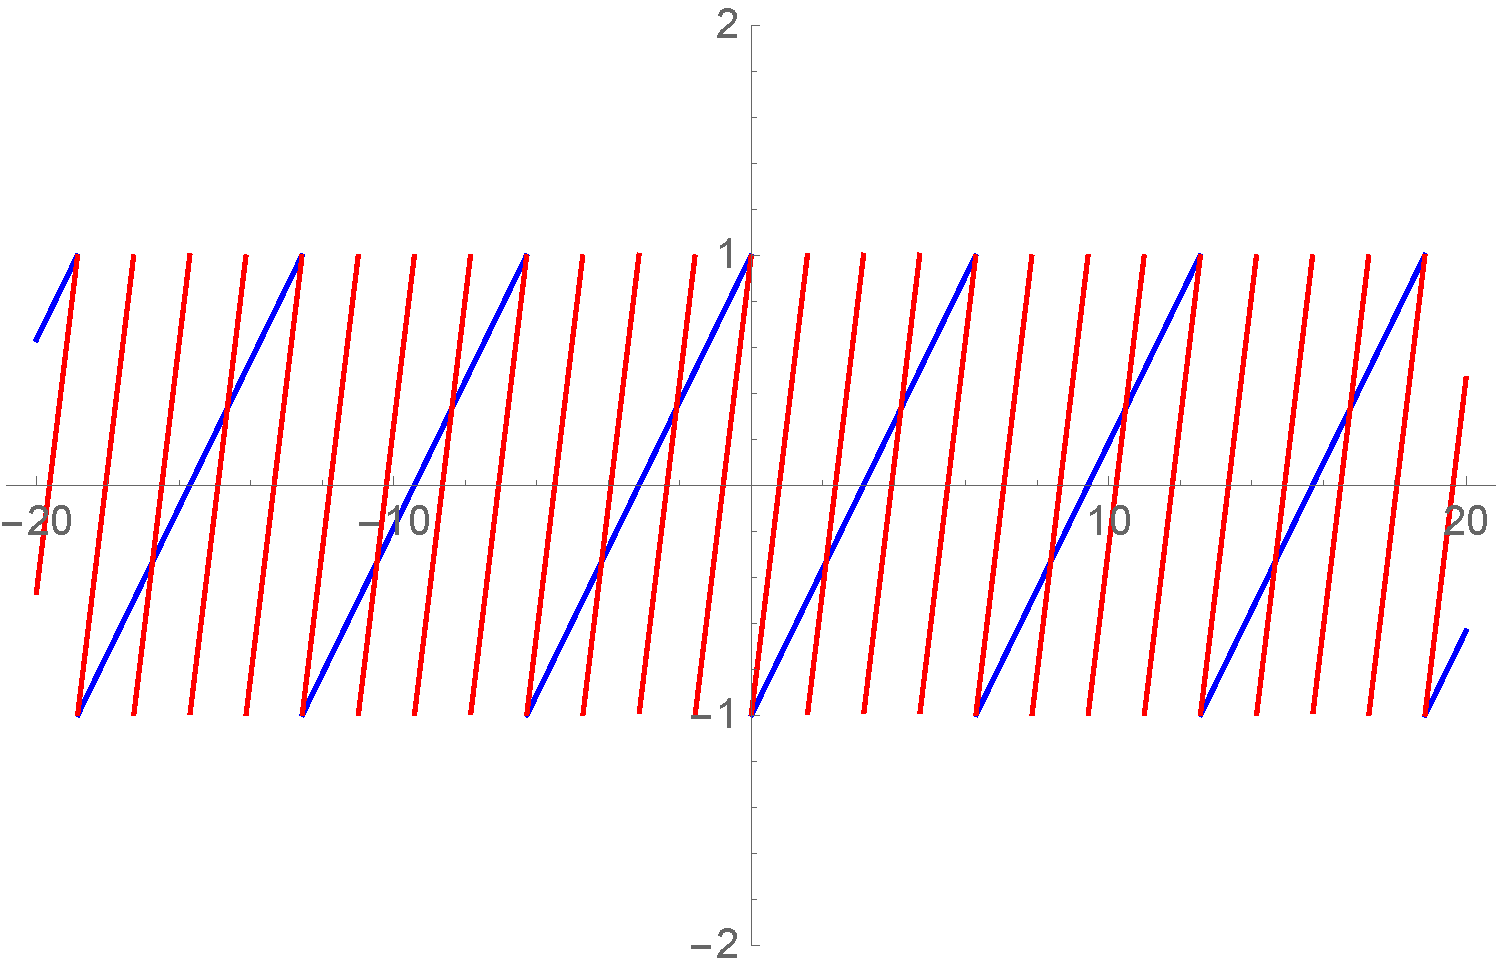
\includegraphics[width=140mm, scale=0.5]{images/sawtooth-comparison.pdf}
  \caption{Graph of 2 sawtooth functions with different periods. The blue function has a longer period, while the red function has a shorter period.}
  \label{Sawtooth-comparison}
\end{figure}

\begin{figure}[H]
  \centering
  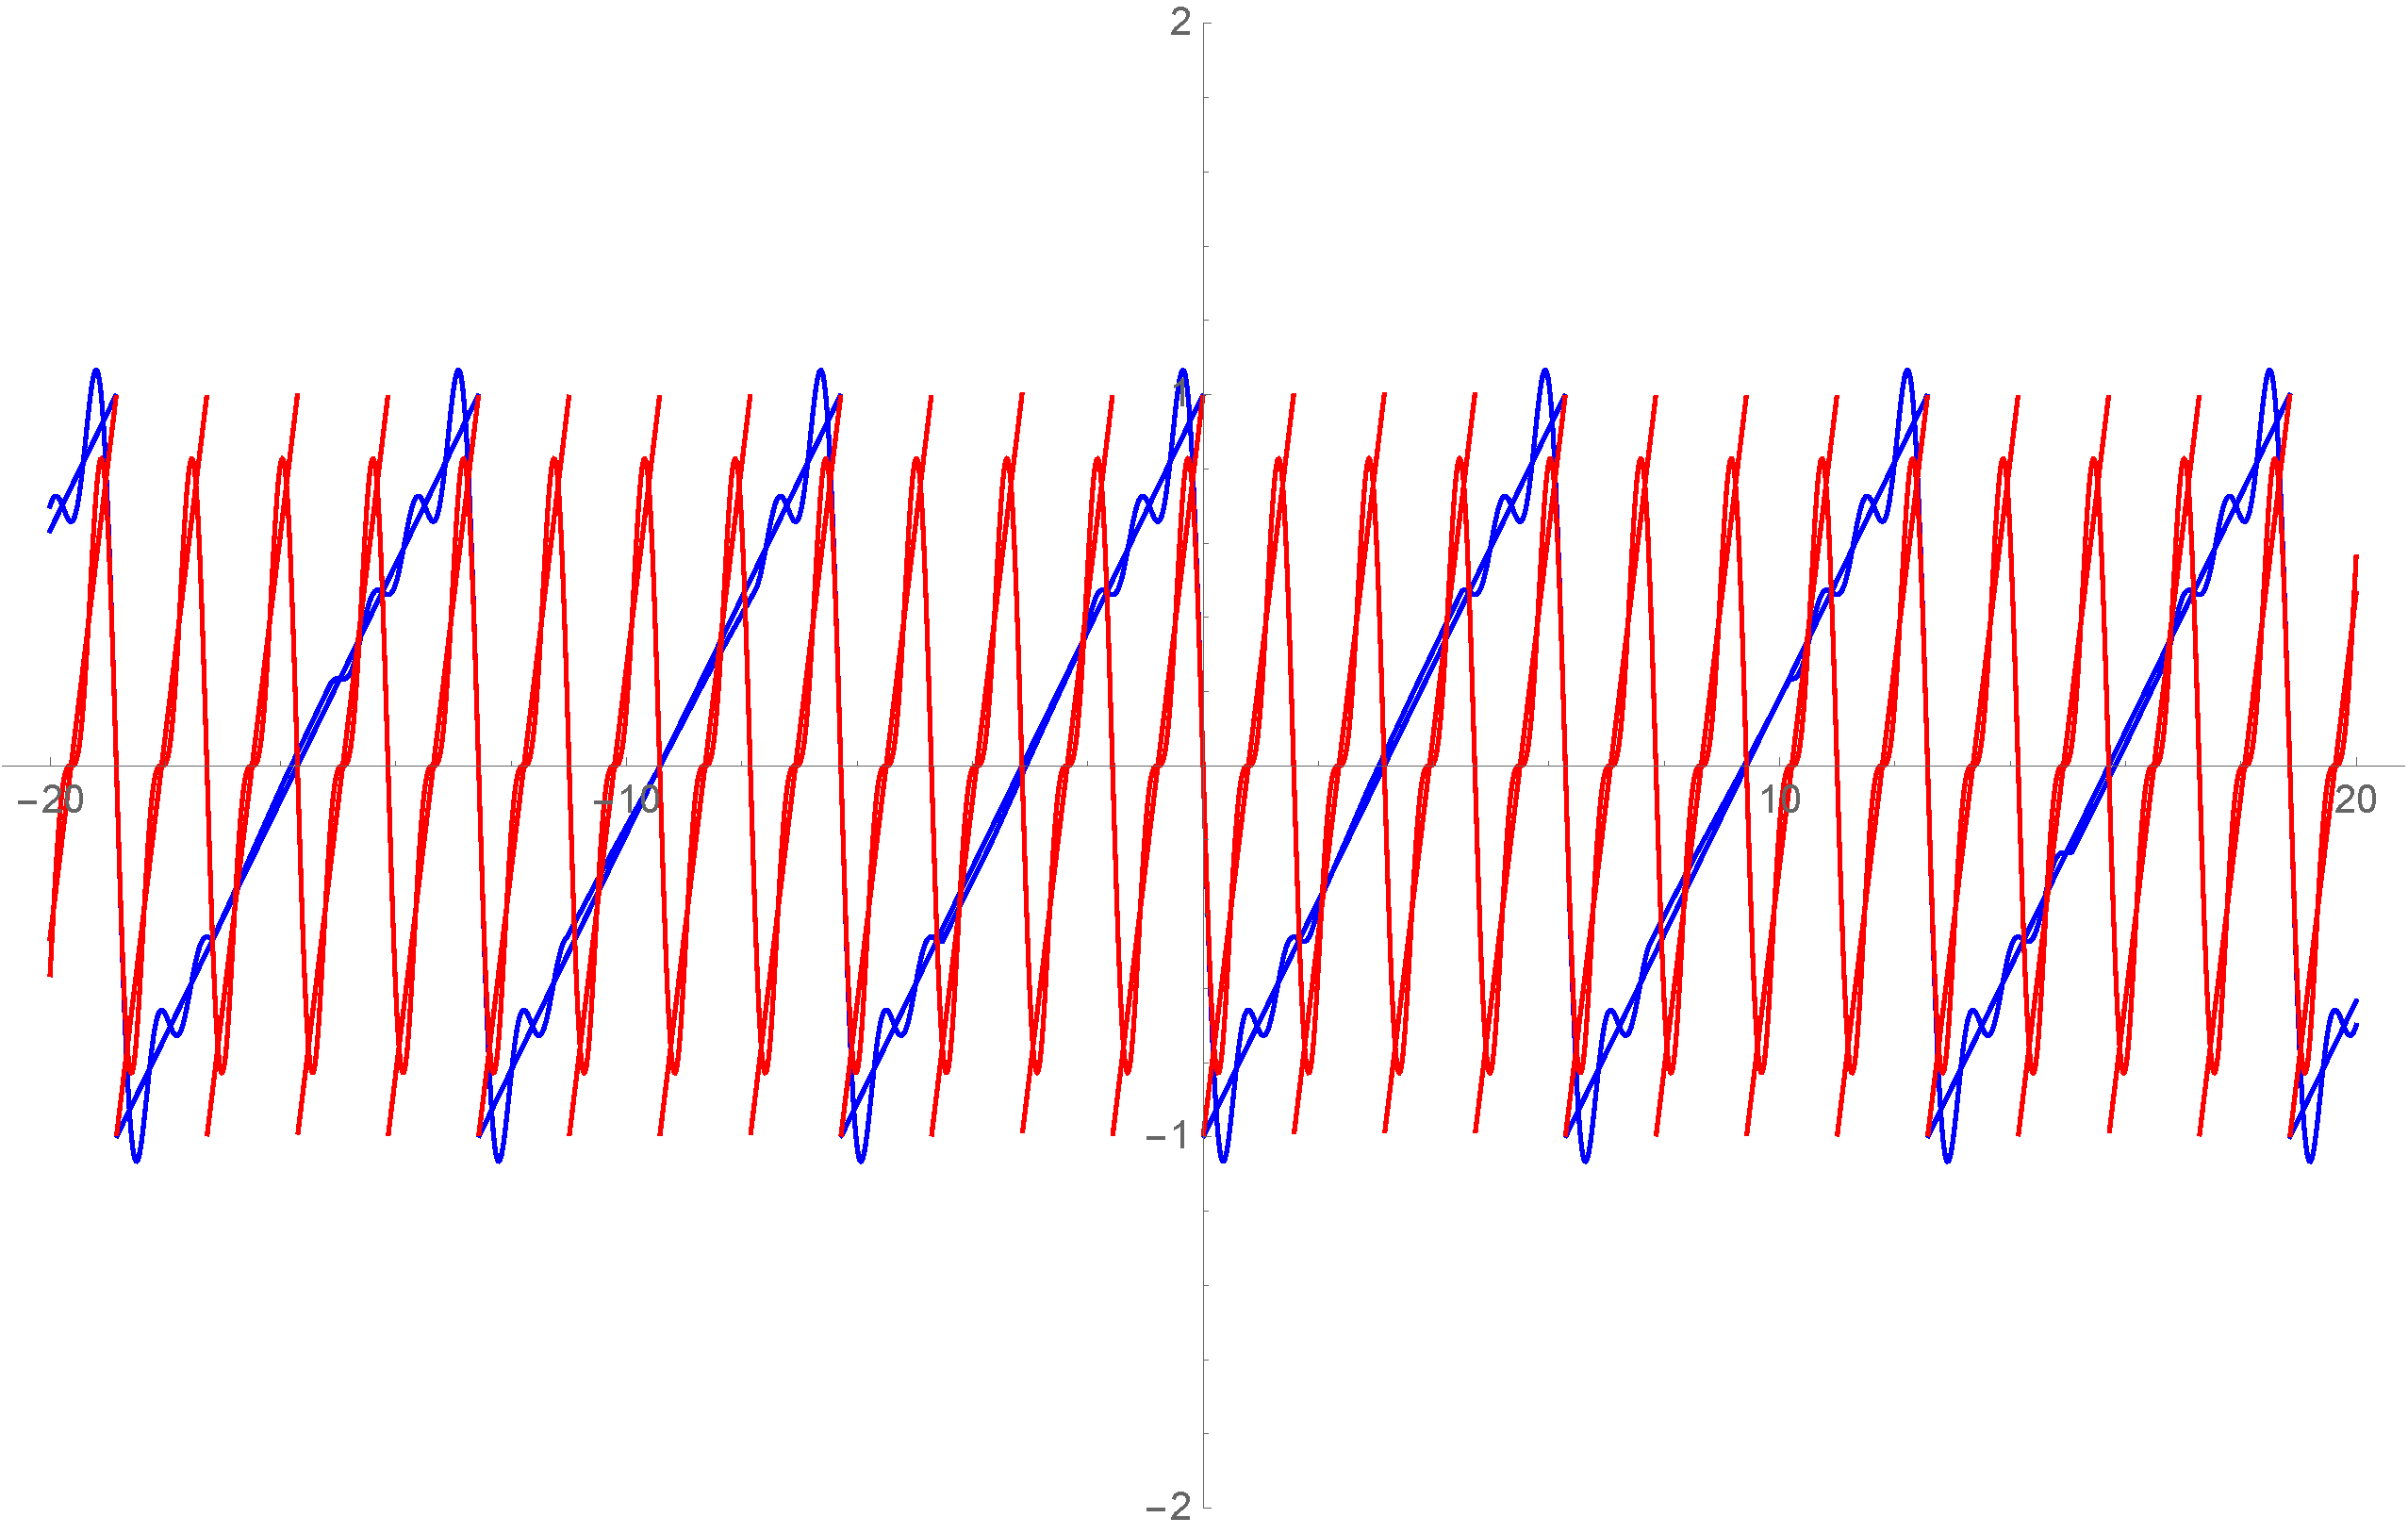
\includegraphics[width=140mm, scale=0.5]{images/sawtooth-comparison-real-space.pdf}
  \caption{Graph of 2 sawtooth functions approximated with the first few terms of their Fourier series (real space)}
  \label{Sawtooth-comparison-real-space}
\end{figure}


\begin{figure}[H]
  \centering
  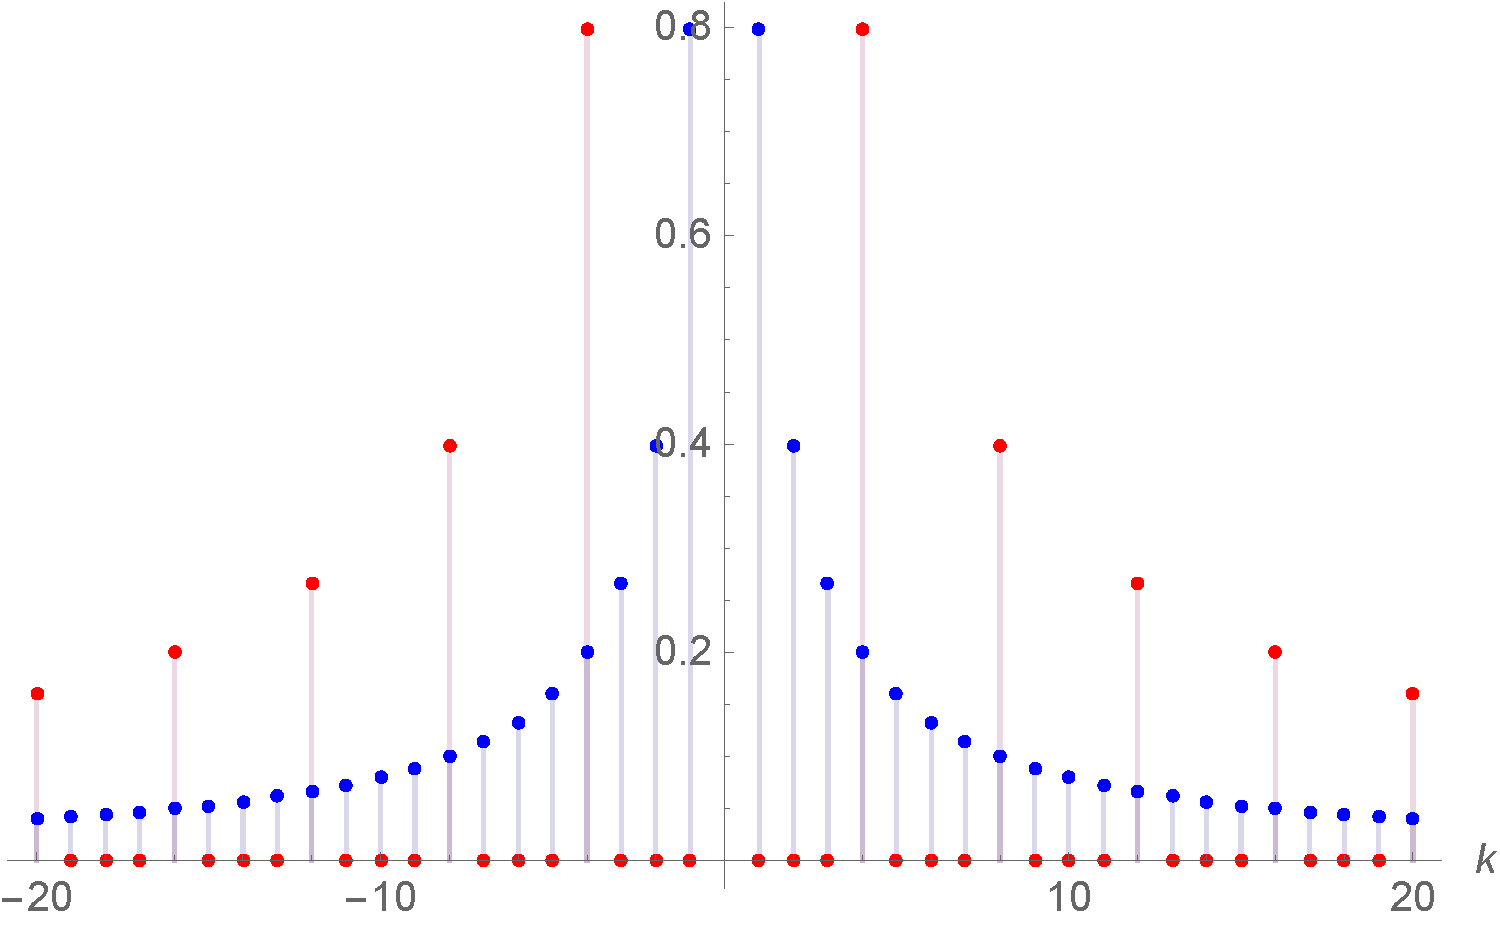
\includegraphics[width=140mm, scale=0.5]{images/sawtooth-comparison-k-space.pdf}
  \caption{Graph of 2 sawtooth functions in Fourier k-space}
  \label{Sawtooth-comparison-k-space}
\end{figure}



\end{document}
